\documentclass[MASTER.tex]{subfiles} 
\begin{document} 
\begin{frame}
	\begin{figure}
		\centering
		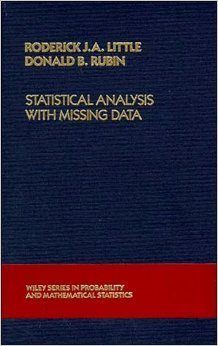
\includegraphics[width=0.45\linewidth]{LittleRubin}
	\end{figure}
	
\end{frame}
%====================================================== %
\begin{frame}
	\frametitle{What is multiple imputation?}
	\Large
\noindent \textbf{Imputation}
\begin{itemize}
\item 	Imputation, the practice of '\textit{filling in}' missing data with plausible values, is an attractive approach to analyzing incomplete data. 
\item The intention is to solve the missing-data problem at the beginning of the analysis.
\item However, a naive or unprincipled imputation method may create more problems than it solves, distorting estimates, standard errors and hypothesis tests, as documented by Little and Rubin (1987) and others.
\end{itemize}
\end{frame}
%====================================================== %
\begin{frame}
	\Large
	\noindent \textbf{Imputation}
	\begin{itemize}
\item For \textbf{MNAR}, imputation is not sufficient, because the missing data are totally different from the
available data, i.e. your complete data has become a selective group of persons. 
\item For \textbf{MCAR} and \textbf{MAR}, there are roughly two kinds of techniques for imputation; Single and Multiple
Imputation.
	\end{itemize}


\end{frame}
%====================================================== %
\begin{frame}
	\frametitle{Single Imputation}
	\Large
\noindent \textbf{Single Imputation}
\begin{itemize}
\item Single imputation techniques are based on the idea that in a random sample every person can be
replaced by a new person, given that this new person is randomly chosen from the same source
population as the original person. 
\item In that case you can use the observed available data of the
other persons to make an estimation of the distribution of the test result in the source population.
\item It is called \textbf{single imputation}, because each missing is imputed once.
\end{itemize}

\end{frame}
%====================================================== %
\begin{frame}
	\frametitle{What is multiple imputation?}
	\Large
\begin{itemize}
\item There are many methods for single imputation, such as {
	\LARGE
	\begin{itemize}
\item replacement by the mean, 
\item regression,
\item expected maximization (EM). 
\end{itemize}
}
\item \textbf{Expected maximization} is preferred, because in the other methods
the variance and standard error are reduced and the chance for Type II errors increases. 
\end{itemize}

\end{frame}

\begin{frame}
	\frametitle{Multiple Imputation}
\Large
\begin{itemize}
\item	Multiple imputation is a simulation-based approach to the statistical analysis of incomplete data. 
\item In multiple imputation, each missing datum is replaced by $m>1$ simulated values. 
\item The resulting m versions of the complete data can then be analyzed by standard complete-data methods, and the results combined to produce inferential statements (e.g. interval estimates or p-values) that incorporate missing-data uncertainty.
\end{itemize}	
	
\end{frame}
%http://sites.stat.psu.edu/~jls/mifaq.html

%====================================================== %
\begin{frame}
	\frametitle{What is multiple imputation?}
	\Large
\begin{itemize}
\item The difference with single imputation is that in MI the value is imputed for several times. There are
more imputed datasets created. 
\item The different imputations are then based on random draws of
different estimations of the underlying distribution in the source population. 
\item In this way, the
imputed data comes from different distributions and therefore are less look alike. 
\item There is more
uncertainty created in the dataset. Therefore the standard error increases. 
\end{itemize}

\end{frame}
%====================================================== %
\begin{frame}
	\frametitle{What is multiple imputation?}
	\Large 
\begin{itemize}
\item The amount of
imputations is dependent on the amount of missing data, but mostly 5 to 10 imputations are
enough. 
\item A drawback of this method it that several imputed datasets are created and that the
statistical analysis has to be repeated in each dataset. \item Finally, results have to be pooled in a
summary measure. Most statistical packages can do this automatically.
\end{itemize}
\end{frame}
%============================================= %




	%====================================================== %
	\begin{frame}
		\frametitle{Multiple Imputation}
		\Large
\begin{itemize}
\item The question of how to obtain valid inferences from imputed data was addressed by Rubin's (1987) book on multiple imputation (MI).
\item MI is a Monte Carlo technique in which the missing values are replaced by $m>1$ simulated versions, where $m$ is typically small (e.g. 3-10). 
\end{itemize}

	\end{frame}

	%====================================================== %
	\begin{frame}
\frametitle{Multiple Imputation}
		\Large
		\begin{itemize}
\item In Rubin's method for `\textbf{repeated imputation}' inference, each of the simulated complete datasets is analyzed by standard methods, and the results are combined to produce estimates and confidence intervals that incorporate missing-data uncertainty.
\item  Rubin (1987) addresses potential uses of MI primarily for large public-use data files from sample surveys and censuses. 
		\end{itemize}

	\end{frame}
	%====================================================== %
	\begin{frame}
		\frametitle{Multiple Imputation}
		\Large
	\begin{itemize}
\item With the advent of new computational methods and software for creating MI's, however, the technique has become increasingly attractive for researchers in the biomedical, behavioral, and social sciences whose investigations are hindered by missing data. 
\item These methods are documented in a recent book by Schafer (1997) on incomplete multivariate data.
	\end{itemize}

\end{frame}
\end{document}
